\documentclass[11pt]{article}

% BASIC PACKAGES
\usepackage{latexsym}
\usepackage{amssymb,amsmath,pgf,graphicx,bm}
\usepackage{amsthm}
\usepackage{thmtools}

% FONTS AND SPACING
\usepackage{amsfonts}
\usepackage{tgpagella} % font
\usepackage[margin=0.8in]{geometry}
\usepackage{setspace}
\usepackage{caption}
%\onehalfspacing % or
\doublespacing

% SPECIAL FORMATTING
\usepackage{fancyhdr}
\usepackage[T1]{tipa} % for ipa
\usepackage{color}
\usepackage{tabulary}
\usepackage{mdframed}
\usepackage{algpseudocode}
\usepackage{tikz}

% MATHEMATICAL COMMANDS
\DeclareMathOperator*{\argmax}{arg\,max}
\newcommand{\bvec}[1]{\vec{\mathbf{#1}}}
\newcommand{\R}{\mathbb{R}}
\newcommand{\overlap}{\textsc{Overlap}}
\newcommand{\lkhd}{\textsc{Likelihood}}
\newcommand{\goodaction}{\textsc{GoodAction}}

% DEFINITIONS, THEOREMS, & CLAIMS
\newtheorem{theorem}{Theorem}
\declaretheorem[style=definition,qed=$\blacksquare$]{definition}
\newenvironment{claim}[1]{\par\noindent\textit{Claim.}\space#1}{\hfill $\blacksquare$}

\pagestyle{fancy}
\fancyhf{}
\rhead{\today}
\lhead{Jennifer Hu}
\cfoot{\thepage}

\begin{document}

\begin{center}
\Large{Finding optimal goals in card games with uncertainty}
\end{center}

\section{Introduction}

Given the history of the card game, what is the optimal goal to pursue? By building a bot that can answer this question at every step of the game, we can evaluate human players' performance, rationality, and goal-oriented language in a systematic way.

In a standard 52-card deck, there are 52 possible straight flushes of 6 cards. Each of these 6-card straight flushes is called a goal, and we give weights to each of them in the vector $\bvec{w} \in \R^{52}$, which is updated every time we learn new information about the game. Before any cards are dealt, every goal is equally (un)optimal, and $\bvec{w} := \bvec{0}$. The game history contains information about the number of cards reshuffled at each round and the cards we have already seen.

\section{The Features}

When expert humans play the game, they tend to evaluate goals based on three features: (1) how many visible cards (i.e. in the hands and table) coincide with the goal, (2) how likely it is to obtain the goal based on which cards might have already been discarded, and (3) how much closer their range of possible actions can bring them to the goal during their turn. I call these features $\overlap$, $\lkhd$, and $\goodaction$, respectively.

\subsection{$\overlap$}

$\overlap$ measures how many cards in common a certain goal $G$ has with a set of cards $C$. Formally, $\overlap$ is defined as the following:
\begin{equation}
\overlap(G,C) = |G \cap C|
\label{eq:overlap} \end{equation}
$\overlap$ takes on values in the interval $[0,6]$. It is independent of game history.

Another way of thinking of $\overlap$ is that $6-\overlap(G,C)$ represents the number of cards ``away'' $C$ is from goal $G$.

\subsection{$\lkhd$}

$\lkhd$ measures how likely it is that a certain goal $G$ can be obtained given all previous history $H$. $\lkhd$ is defined as the following:
\begin{align}
  \mathcal{L}(G,H) &= \prod_{g \in G} P(g \text{ is still in play}|H)
  % \mathcal{L}(G,H) &= \sum_{g \in G} \log(1 - P(g \text{ has been discarded}|H))
\end{align}

Given a card $g$ and history $H$, we can find $P(g \text{ is still in play}|H) = 1 - P(g \text{ has been discarded}|H)$ in the following way. First, we know $H$ contains information about $r_i$, the number of cards reshuffled at round $i$ for all $i$, as well as which cards we have and have not seen. Let $s$ be the index of the round that $g$ was last seen, let $n$ be the number of rounds that have occurred between $s$ and now, and let $D_i$ be the size of the deck at round $i$.

\begin{claim}
\begin{equation}
P(g \text{ has been discarded}|H) = \begin{cases}
  0 & g \in \text{ hands or table, or unseen} \\
  \frac{4-r_s}{4-r_s+r_s\prod_{j=1}^n(1-4/{D_{s+j}})} & \text{o.w.}
\end{cases}
\label{eq:p-discarded} \end{equation}
\end{claim}

\begin{proof}
  It is easy to see that a card $g$ cannot have been discarded if it is currently in the hands, on the table, or unseen (in the deck). Now, consider the case where $g$ has not been seen for $n$ rounds (i.e. since round $s$). Let $F$ be the event that $g$ was discarded at round $s$, and let $U$ be the event that $g$ hasn't been seen for $n$ rounds. By the law of total probability, we have
\begin{equation}
  P(F) = P(F|U)P(U) + P(F|U^c)P(U^c).
\label{eq:lotp} \end{equation}

The second term gives us $0$, because if it is not the case that $g$ hasn't been seen for $n$ rounds, then $g$ couldn't have been discarded at round $s$. Consider only the first term. By Bayes' Rule, we have:
\begin{align}
  P(F|U) &= \frac{P(U|F)P(F)}{P(U)} \\
  &= \frac{(1)\left(\frac{4-r_s}{4}\right)}{P(U|F)P(F) + P(U|F^c)P(F^c)} \\
  &= \frac{(4-r_s)/4}{(4-r_s)/4 + (r_s/4)P(U|F^c)}
\end{align}

Let's look at $P(U|F^c)$. Since we are conditioning on $F^c$, we know that $g$ was reshuffled in round $s$, and the size of the deck was updated to $D_s$. The probability of not drawing $g$ in the next round $s+1$ was
\begin{equation}
  \frac{{D_{s+1}-1 \choose 4}}{{D_{s+1} \choose 4}} = \frac{D_{s+1}-4}{D_{s+1}},
\end{equation} and this pattern continued for every subsequent round until the current round $s+n$. This gives us
\begin{equation}
  P(U|F^c) = \prod_{j=1}^n \frac{D_{s+j} - 4}{D_{s+j}}.
\end{equation}

Using this result and simplifying, we finally obtain
\begin{equation}
  P(F|U) = \frac{4-r_s}{4-r_s+r_s\prod_{j=1}^n(1-\frac{4}{{D_{s+j}}})}.
\end{equation}

Plugging this back into (\ref{eq:lotp}), we are left with $\frac{4-r_s}{4}$. This makes intuitive sense. \end{proof}

% See (\ref{eq:decksize}) for an expression for the deck size at each round.

\subsubsection{Deck Size}

It is useful to keep track of the size of the deck at each round $k$ in order to calculate the relevant probabilities. Before any cards are dealt (i.e. round $k=0$), the deck has 52 cards.

\begin{claim}
The size of the deck at round $k > 0$ is given by
\begin{equation}
  D_k = 46 + \sum_{i=1}^{k-1} r_i - 4k.
\label{eq:decksize} \end{equation}
\end{claim}

\begin{proof}
  In the base case, $k=1$ yields $46+0-4(1) = 42$, which is correct since we deal 10 cards from the original 52 in the first round and no cards are reshuffled. Suppose now that (\ref{eq:decksize}) is true for $k=n$. Then we have:
    \begin{align}
      D_{n+1} &= D_n + r_n - 4 \\
      &= (46 + \sum_{i=1}^{n-1} r_i - 4n) + r_n - 4 \\
      &= 46 + \sum_{i=1}^n r_i - 4(n+1)
    \end{align}
  By induction, (\ref{eq:decksize}) holds for all values of $k$. Once $D_k \leq 0$, the game is over.
\end{proof}

\subsection{$\goodaction$}

With $\overlap$ and $\lkhd$, the goal agent gives a good sense of which goals are optimal at each step, but it treats both players' hands as a single object and does not reason about goals using the knowledge that each player must alternate turns. $\goodaction$ incorporates turn-taking into the goal evaluation model. As expert humans, we've found this to be the most challenging part of the game and the primary impetus for goal-changing.

I define $\goodaction$ as the following:
\begin{equation}
  \goodaction(G) = T_1 \cdot A_1(G) + T_2 \cdot A_2(G),
\label{eq:goodaction} \end{equation}
where $T_i$ and $A_i$ are defined as
\begin{align}
  T_i &= \begin{cases}
    1 & \text{currently Player $i$'s turn} \\
    0 & \text{o.w.}
  \end{cases} \\
  A_i(G) &= \max\{\text{all possible improvements Player $i$ can make towards $G$}\}
  % A_i(G) &= \begin{cases}
  %   1 & \exists \text{ an action Player $i$ can take that will bring them closer to $G$} \\
  %   0 & \text{o.w.}
  % \end{cases}
\end{align}

An ``action'' is defined as a swap of 1, 2, or 3 cards between a player's hand and the table. Getting ``closer'' to a goal $G$ is equivalent to increasing the $\overlap$; similarly, the ``improvement'' towards a goal is the change in $\overlap$ after completing the action (the improvement can be negative). Note that $\goodaction(G)$ implicitly depends on the game history $H$ in order to access information about whose turn it is and the players' hands.

\section{Evaluating Goals}

Every time the history $H$ is updated and we observe a new set of cards $C$, the weights $w_i$ for each goal $G_i$ are updated with a linear combination of the features:
\begin{equation}
  w_i := \bm{\alpha} \cdot [\overlap(G_i,C), \lkhd(G_i,H), \goodaction(G_i)]
\label{eq:w-update} \end{equation}

After the weights are updated, the model returns the optimal goal(s), which correspond to the max value(s) in $\bvec{w}$.

\subsection{Player Actions}

A player chooses an action in the following way. First, the player calculates the improvements made by each possible action for each of the optimal goals. If the maximal improvement is nonnegative, then the player performs the action that gives that max improvement. Otherwise, the player calculates the most common suit appearing among the optimal goals and checks if any possible actions will increase the number of cards in their hand with that suit. If no such actions exist, the player executes a randomly chosen action.

% The values of $\bm{\alpha} \in \mathbb{R}^3$ should be set to reflect the agent's preferences. A more human-like agent might weigh $\overlap$ over $\lkhd$, for example, since it tends to consider only the visible cards and does not calculate probabilities based on game history. Expert humans might also be more likely to place greater weight on $\goodaction$, which would be reflected in a high $\alpha_2$ value.

\section{Discussion}

\subsection{Initial Results}

Figure \ref{fig:success} shows the success rates (over 50 trials) for games played for $p \in \{0, 0.25, 0.5, 0.75, 1\}$ and $\bm{\alpha} \in \{[1,1,1], [1,2,3], [1,3,2], [2,1,3], [2,3,1], [3,1,2], [3,2,1]\}$. Success is defined by achieving a 6-card straight flush before the deck runs out of cards.

\begin{figure}[hpt]
  \centering
  \captionsetup{justification=centering,margin=2cm}
  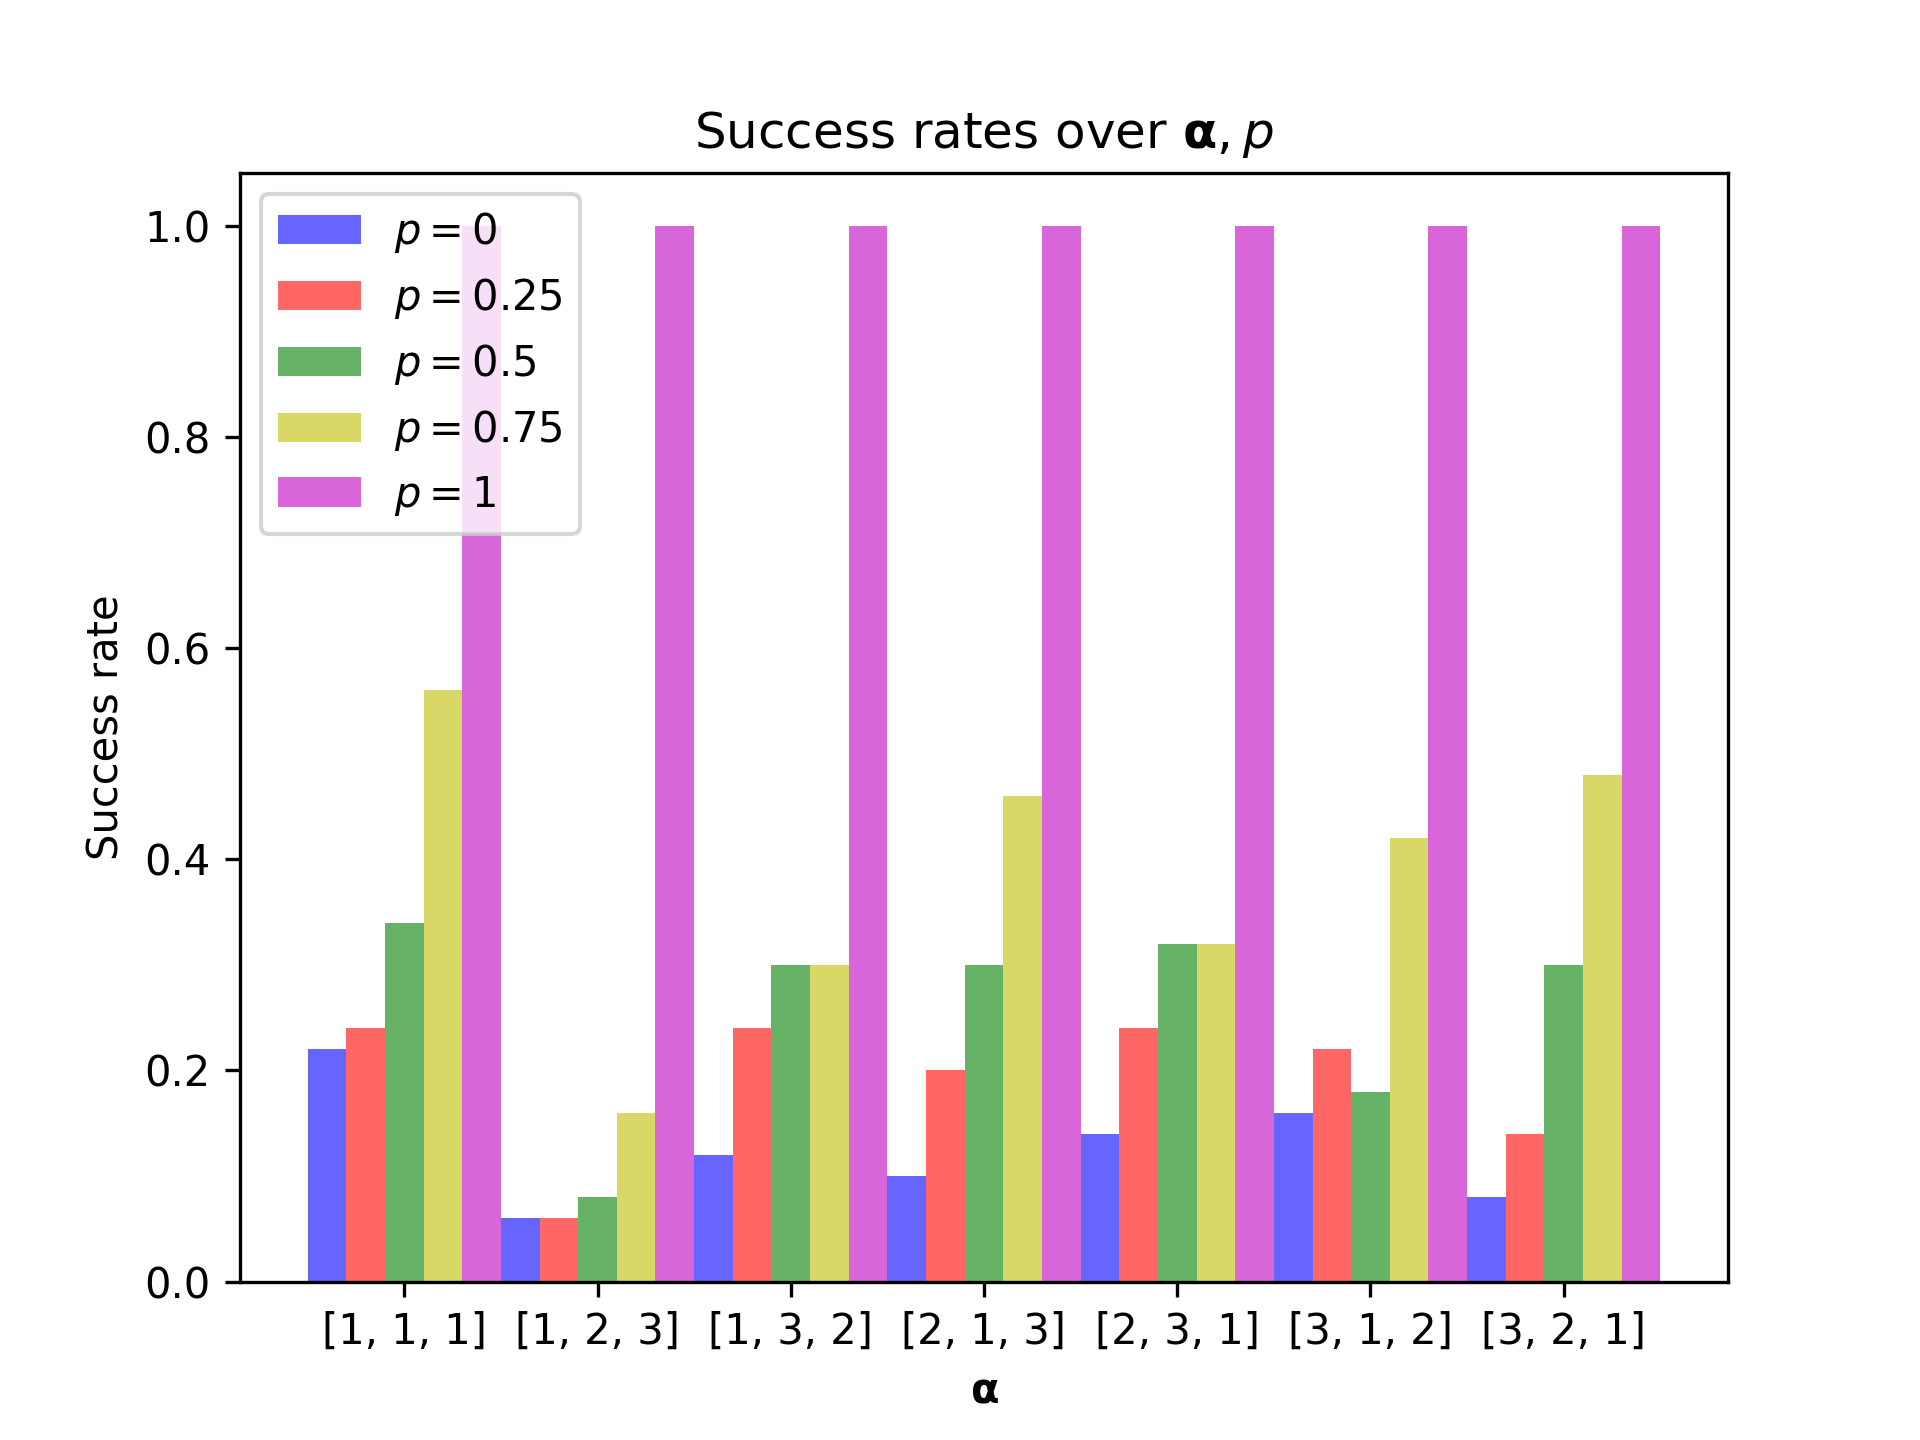
\includegraphics[scale=0.8]{../plots/successAlphaP.png}
  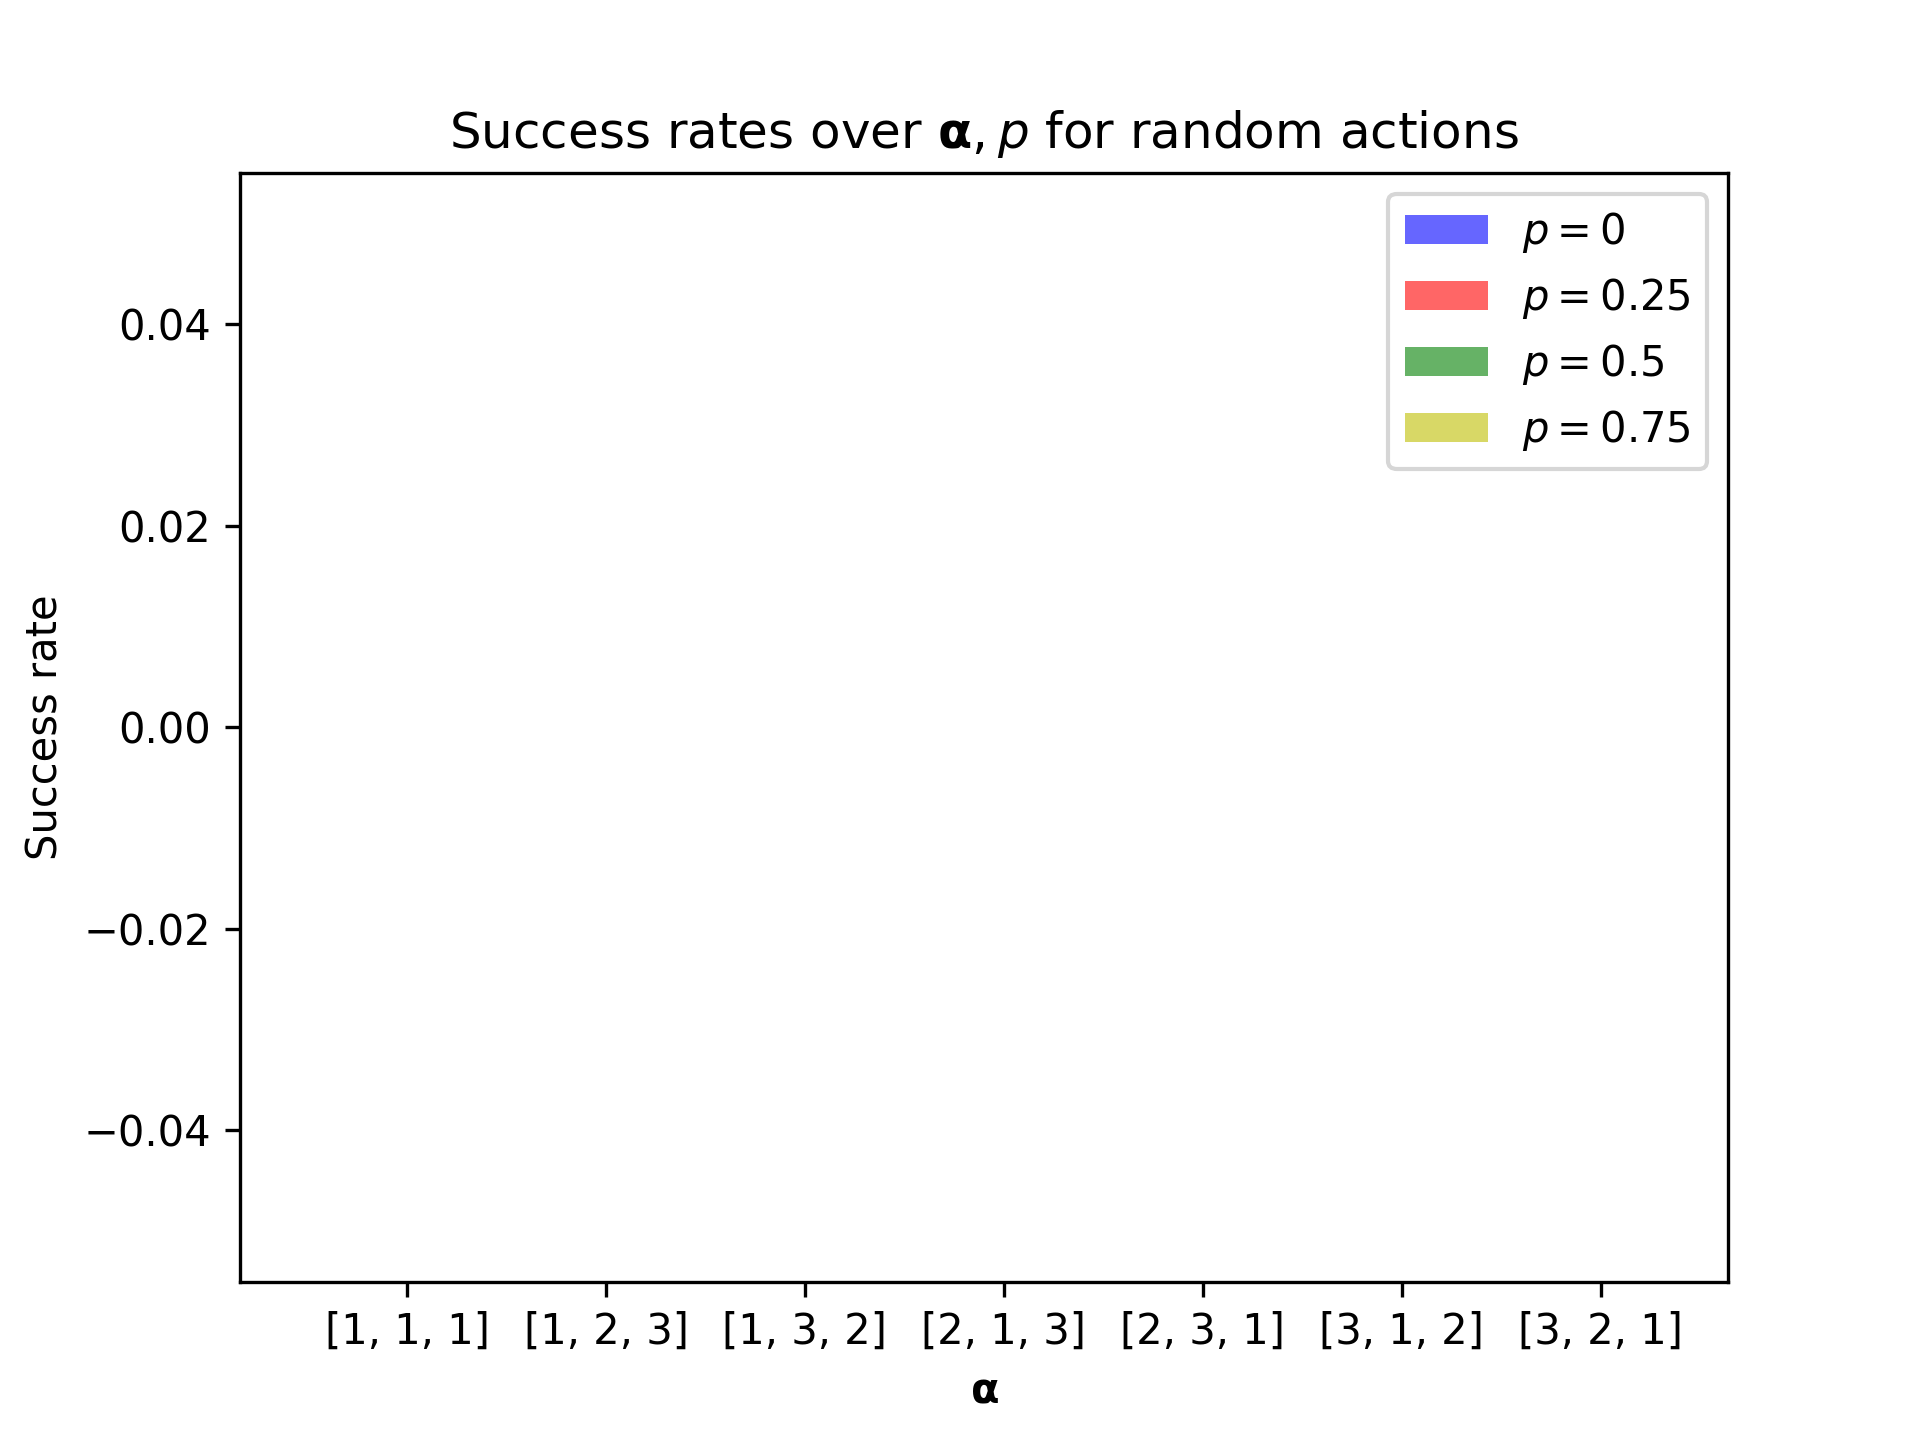
\includegraphics[scale=0.8]{../plots/successAlphaP_RANDOM.png}
  \caption{Success rates across different values of $\bm{\alpha}$ and $p$. The bottom graph shows baseline performance for random player actions with $p=1$ omitted -- the random player lost every game.}
  \label{fig:success}
\end{figure}

As expected, $p=1$ gives a success rate of 1, as the deck never runs out of cards. The success rate increases as $p$ increases, but it doesn't seem to be a linear relationship. Interestingly, the model had best performance when each feature was weighed equally, corresponding to $\bm{\alpha} = [1,1,1]$. $\bm{\alpha} = [2,3,1]$ also seemed to do well across values of $p$, but more trials are needed to robustly compare results.

Figure \ref{fig:rounds} shows the mean number of rounds played per game (over 50 trials) for games played for $p \in \{0, 0.25, 0.5, 0.75, 1\}$ and $\bm{\alpha} \in \{[1,1,1], [1,2,3], [1,3,2], [2,1,3], [2,3,1], [3,1,2], [3,2,1]\}$.

\begin{figure}[hpt]
  \centering
  \captionsetup{justification=centering,margin=2cm}
  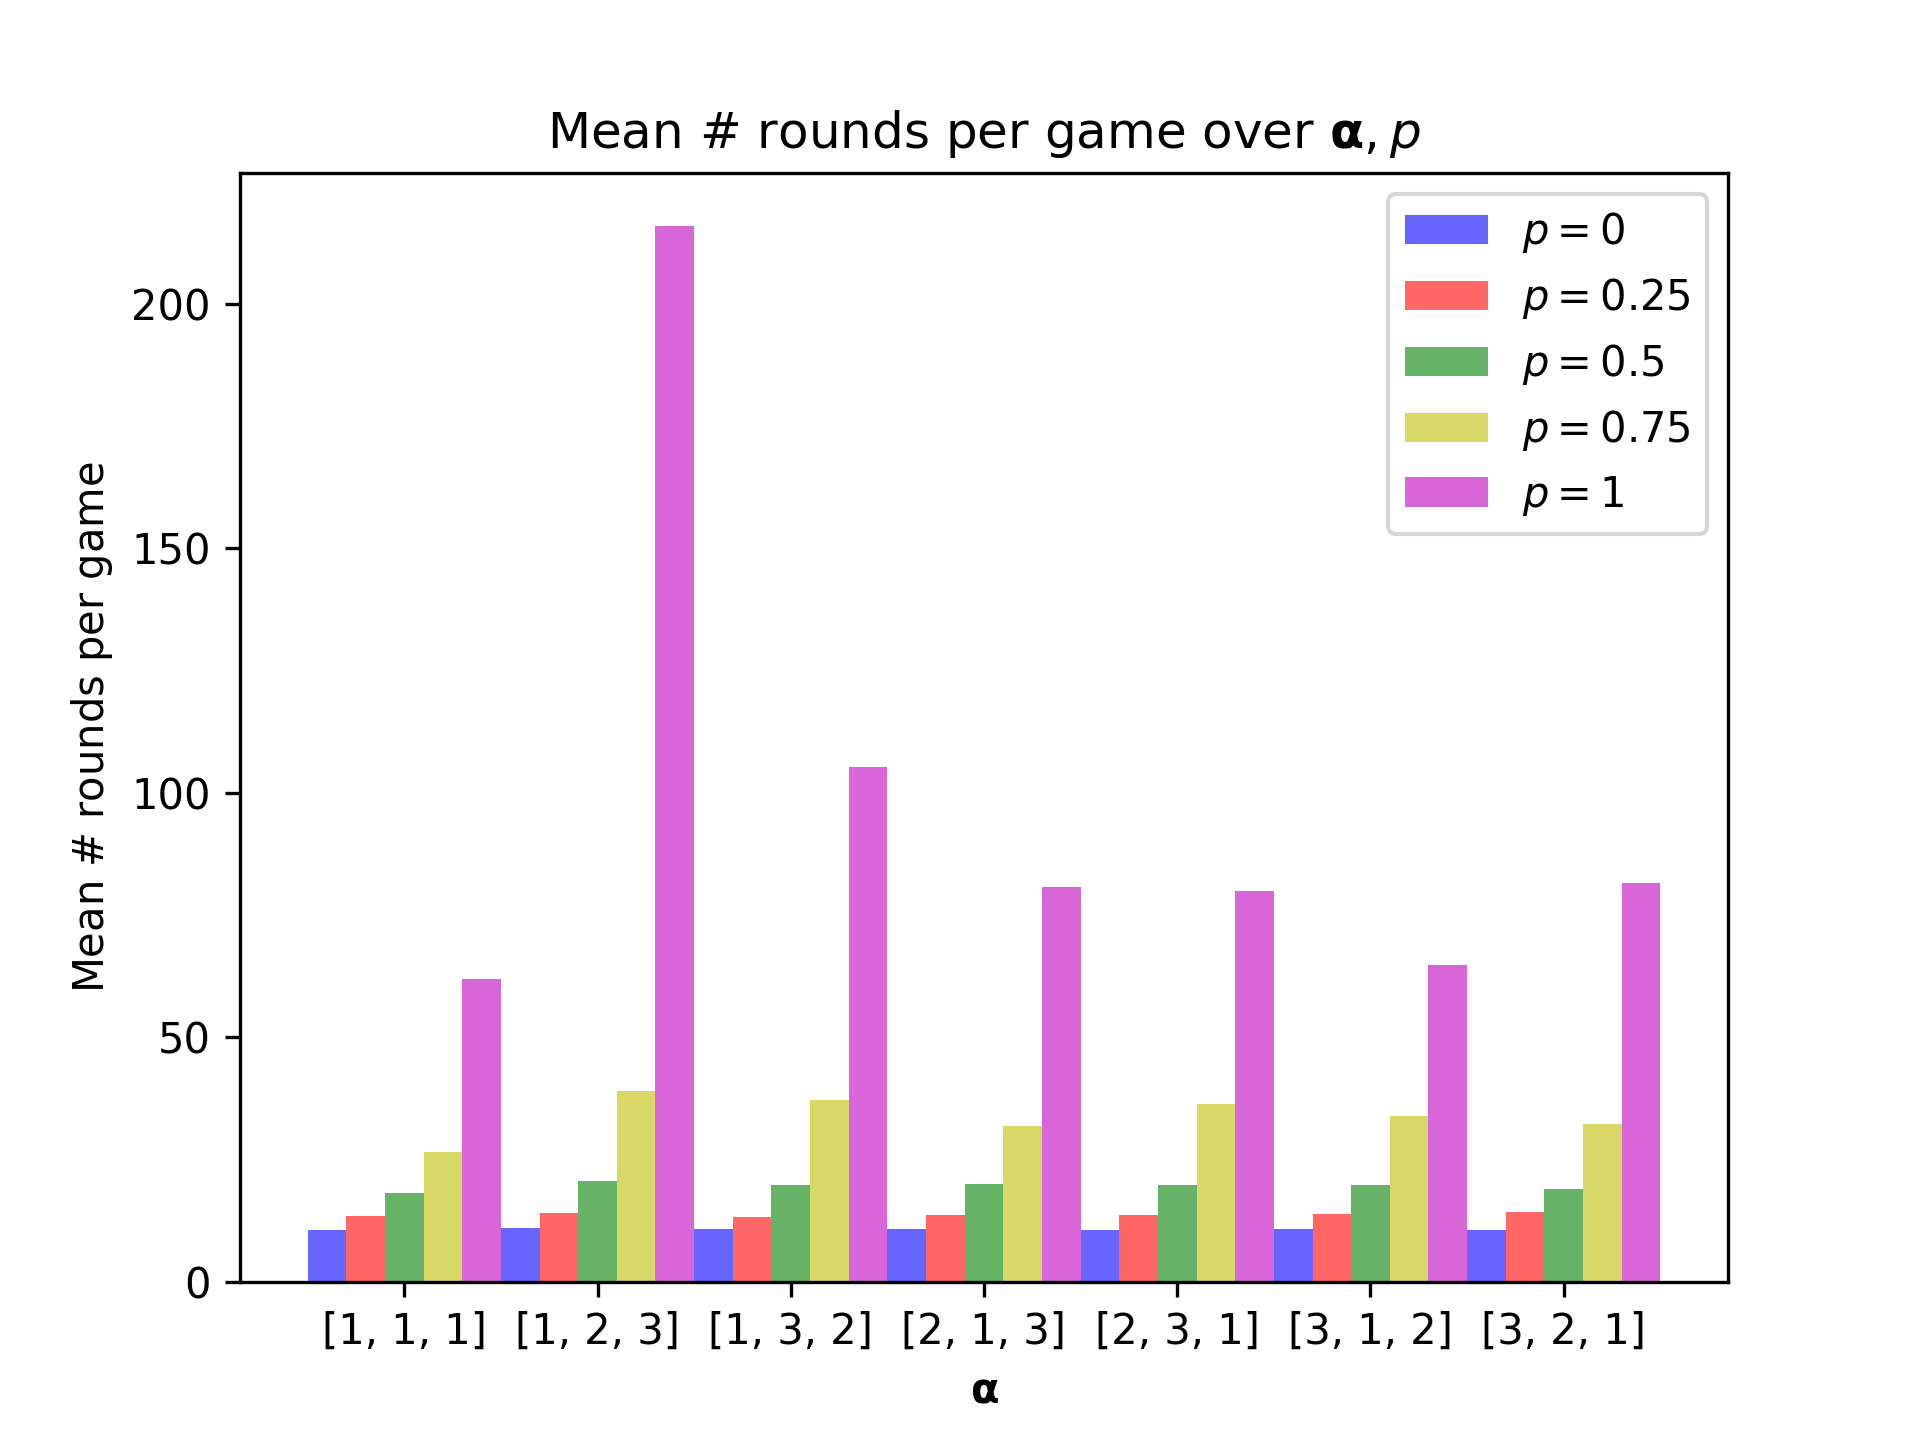
\includegraphics[scale=0.8]{../plots/roundsAlphaP.png}
  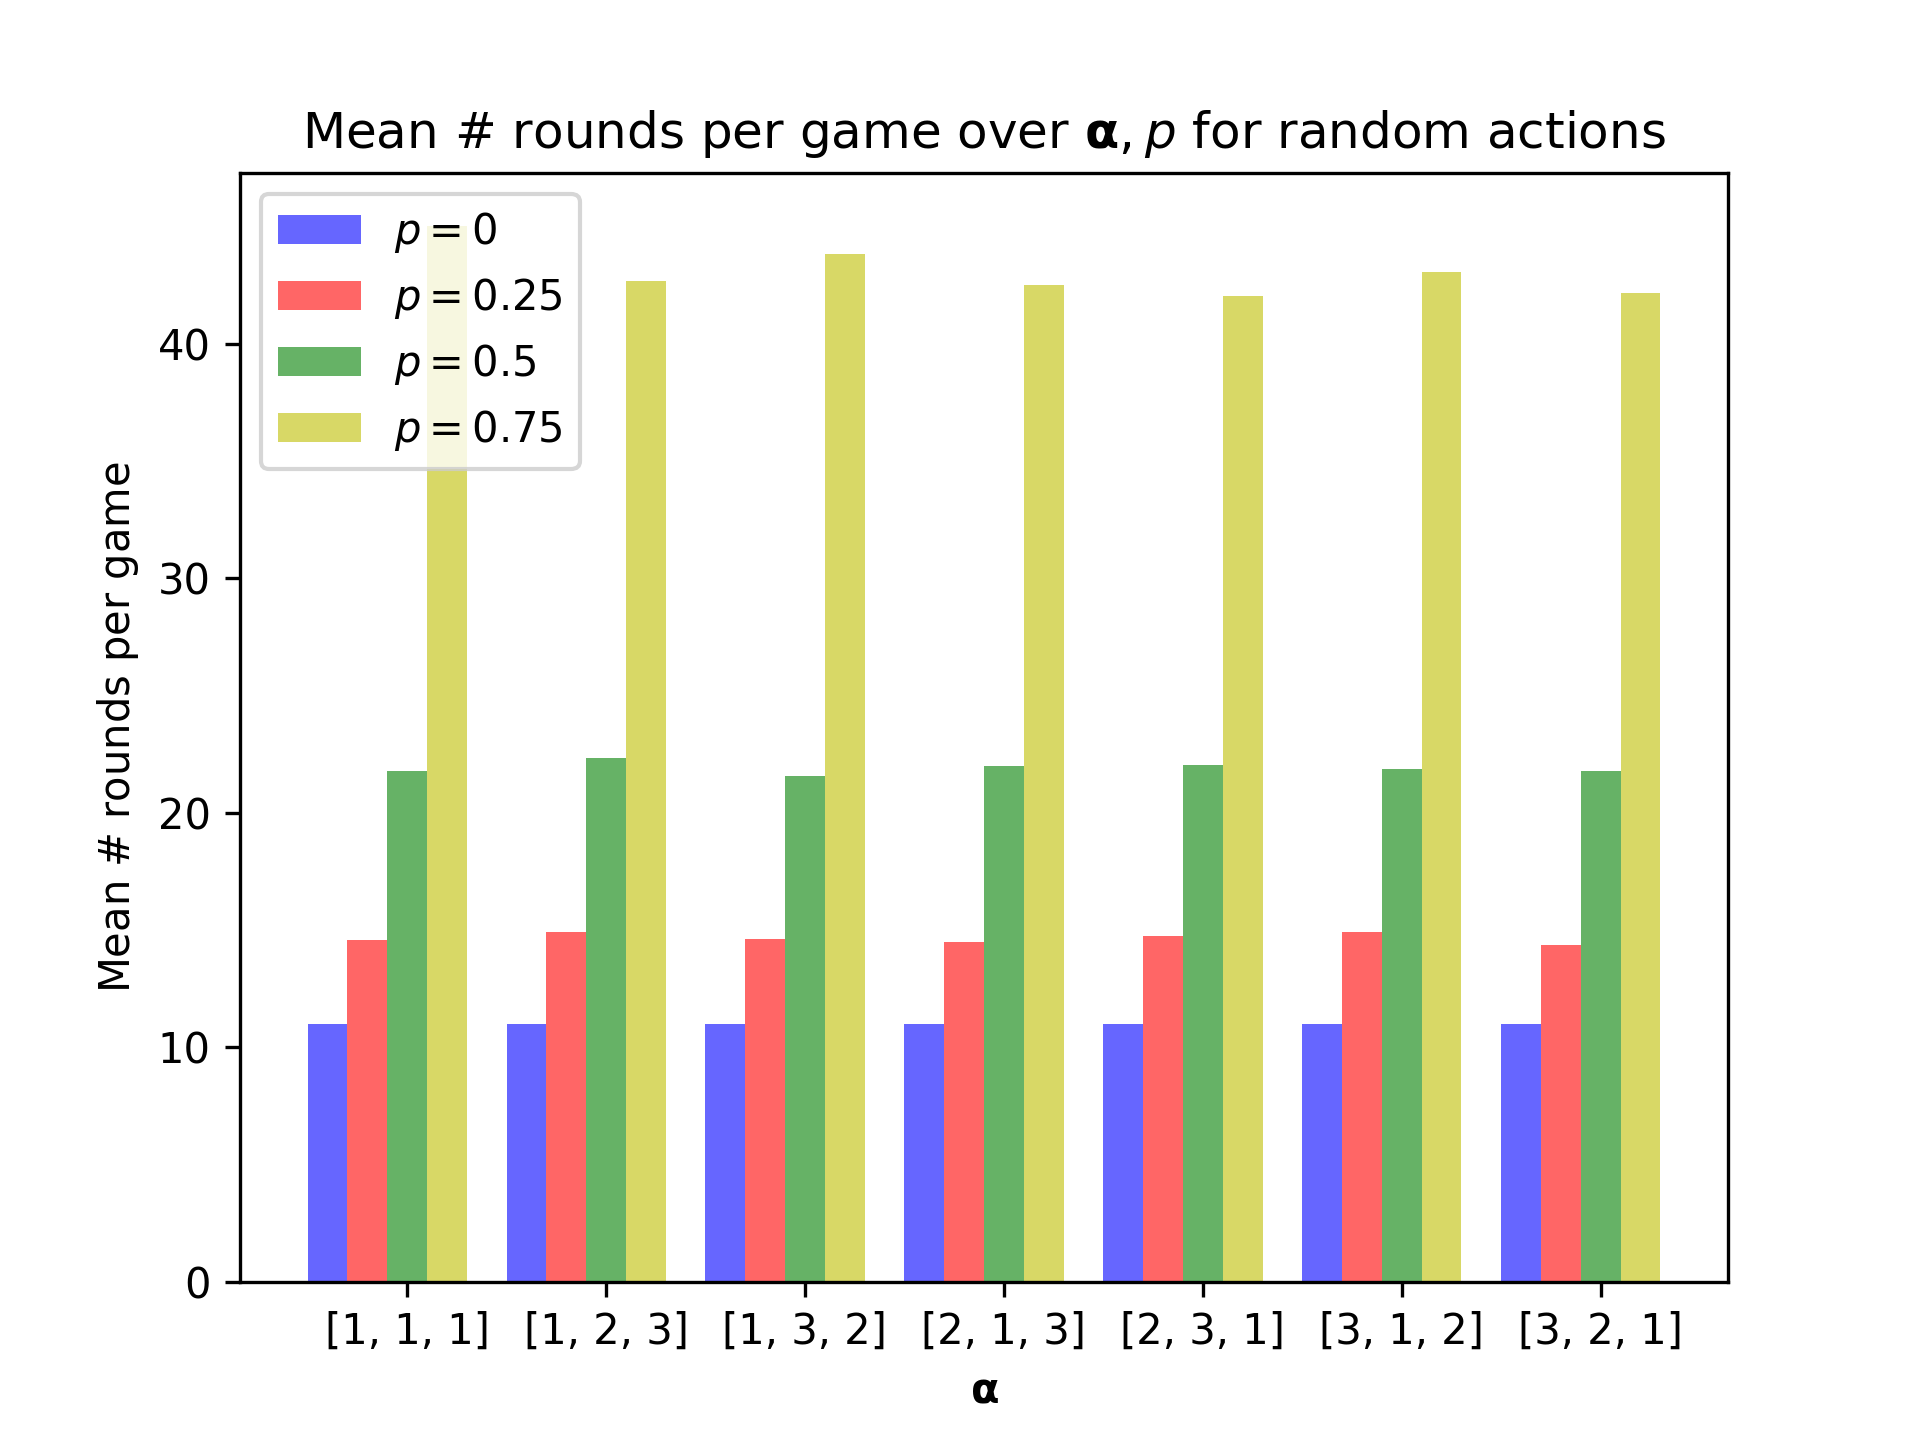
\includegraphics[scale=0.8]{../plots/roundsAlphaP_RANDOM.png}
  \caption{Mean number of rounds across different values of $\bm{\alpha}$ and $p$. The bottom graph shows baseline performance for random player actions with $p=1$ omitted.}
  \label{fig:rounds}
\end{figure}

The number of rounds tends to increase as $p$ increases, as expected. Like the success rates, the number of rates does not seem to increase linearly.

\subsection{Observations}

Although this simple model reflects how humans might approach the card game, it doesn't seem optimal in a ``ground truth'' sense. Ideally, I would like to combine the notions of $\lkhd$ and $\goodaction$, because the likelihood or feasibility of obtaining a goal should depend on the order of turns. On the other hand, having the features separated in this naive way might help us detect changes in human players' intentions as their language changes.

I also need to think more about how players should choose their actions. The greedy algorithm I've written seems reasonable, but still a little bit ad hoc.

\section{POMDPs}

Another approach is to model the problem as a Partially Observable Markov Decision Process (POMDP).

\subsection{States}

We define the set of states to be
\begin{equation}
  S = \{1, 2, 3, 4, 5\}^{52},
\label{eq:states} \end{equation}
where each component $s_i$ of a state $\mathbf{s} \in S$ corresponds to the card $c_i$ in the deck. The value of $s_i$ is determined by
\begin{equation}
  s_i = \begin{cases}
    1 & c_i \in \text{hand 1} \\
    2 & c_i \in \text{hand 2} \\
    3 & c_i \in \text{table} \\
    4 & c_i \in \text{deck} \\
    5 & c_i \in \text{discarded}
  \end{cases}.
\label{eq:statecomponents}\end{equation}

This gives us $5^{52} \approx 2.22 \cdot 10^{36}$ different states. There are about $5.6 \cdot 10^{21}$ grains of sand on Earth.

\subsection{Actions}

The set of actions $A$ includes all possible swaps a player can make with 1, 2, or 3 cards between their hand and the table, as well as an \texttt{END\_TURN} action. Since the active hand has 3 cards and the table has 4 cards, there are

\begin{equation}
  {3 \choose 1}{4 \choose 1} + {3 \choose 2}{4 \choose 2} + {3 \choose 3}{4 \choose 3} = 34
\label{eq:swaps}\end{equation}

possible swaps. Together with \texttt{END\_TURN}, this gives us 35 total actions.

\subsection{Reward}

We can define a simple reward function:

\begin{equation}
  r(s,a) = \begin{cases}
    1 & \text{if you win} \\
    0 & \text{o.w.}
  \end{cases}
\end{equation}

\subsection{Transitions}

\subsection{Observations}

\end{document}
